%!TEX root = ../../csuthesis_main.tex
\chapter{深度强化学习方法}

\section{深度Q网络算法 }

\subsection{深度Q网络算法概述 }

我们可以通过现有的研究自动,深度Q网络(DQN)\cite{mnih2015human}是由 DeepMind 首次在生命科学领域发布的网络架构。它的出现引发了人们的思考,让人们了解到一种新型算法的用处,那就是强化学习。 Q学习算法通过更新值表来更新函数。当动作和状态连续时,动作的空间显著扩大,状态值的空间也不断扩大。在这种情况下,Q学习算法不再使用。 DQN算法的出现优雅地解决了上述问题,并建立了Q学习算法与卷积神经网络之间的首次紧密联系。它逐渐成为深度学习中应用最广泛的强化学习算法之一。

\subsection{深度Q网络算法原理 }

我们可以通过现有的研究发现,在Q测量算法中,激活值是一种描述,观测值也是一种类似的描述,只不过它们的性能指标不同。 Q可以执行值的记忆功能,并更新值。然而,当代理与环境之间存在信息冲突或多个层次时。 Q值不再完全满足衡量价值的要求,使得平等成为一种诅咒。为了解决这个问题,开发了DQN算法,可以有效地对人进行分类。在这项研究中,DQN参与者认为基于游戏的讲故事是环境学习和发展的重要方法。例如,Atari游戏的最大屏幕尺寸为210x160,每个像素有三个通道。这样,每个状态的维度为210×160×3。显然,Q-questioning算法在处理此类数据时不起作用。

这里的“网络”是指利用神经网络来估计非线性函数的Q值。该神经网络的参数为: 表示每一层的Q权重值。图3-1所示的神经网络由两个全连接层和三个卷积层组成。DQN中神经网络的结构如图3-1所示。

\begin{figure}[hbt]
	\centering
	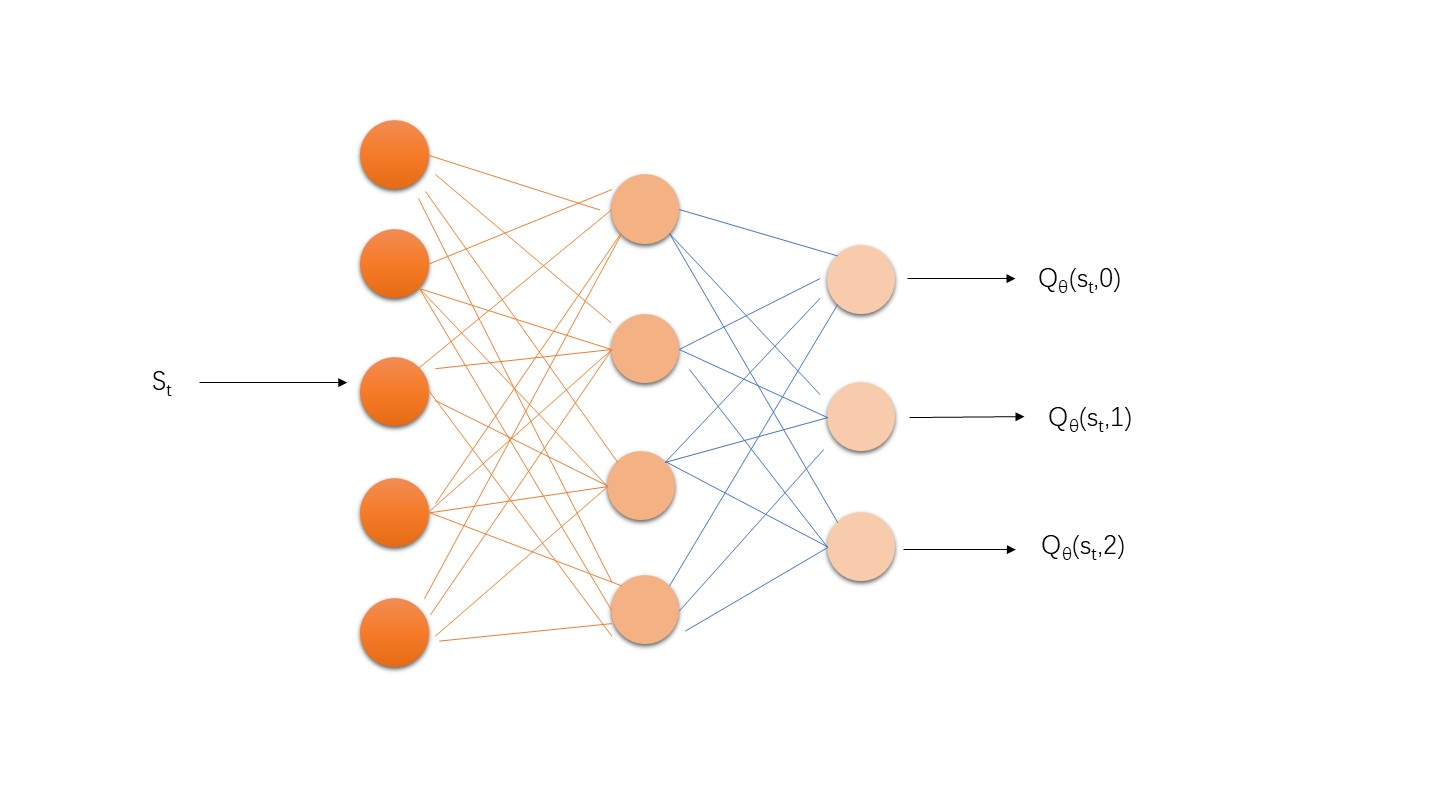
\includegraphics[width=\linewidth]{DQN的深度神经网络结构.jpeg}
	\caption{DQN的深度神经网络结构}
	\label{f.example}
\end{figure}

DQN是一种基于表的新算法。根据算法和变量类型的不同,可分为蒙特卡洛方法和变分方法两类。对应是目标函数为:

\begin{equation}
	\arg\min_{\theta} \left( Q(s,a) - \hat{Q}(s,a,\theta) \right)^2
\end{equation}

在DQN方法中,代价函数往往采用参数的方式来实现。当参数改变时,一方面影响Q值的结果,另一方面也会影响其他值函数。该配置主要基于SGD\cite{wankhadedeep}。设定一个科学的目标来更新和最小化损失函数的值。这里,损失函数本质上是一个量化模型执行与学习过程分布之间差异的函数。在解决实际问题时,不同的问题结构会导致不同形式的功能损失。一般来说,这个问题可以定义为回归问题或分类问题。在回归问题中,最常见的损失函数是L2损失函数(平方误差损失)和L1损失函数。 L2损失函数对与观测值有较大偏差的结果施加较大的惩罚,从而确定结果与真实值的偏差程度;而L1损失函数估计的是真实值和一个比较保守的估计值之间的差值,通常用绝对值来计算。损失函数定义如图表3-1所示。

\begin{table}[htbp]
	\centering
	\caption{损失函数定义}
	\label{tab:loss_functions}
	\begin{tabular}{lll}
		\toprule
		\textbf{回归问题} & \textbf{分类问题} & \textbf{名称} \\
		\midrule
		\(\displaystyle L_1(y, \hat{y}) = w(\theta) | \hat{y} - y |\) & 
		\(\displaystyle L(y, \hat{y}) = -y \log(\hat{y}) - (1-y) \log(1-\hat{y})\) & 
		\multirow{2}{*}{交叉熵损失函数} \\
		
		\(\displaystyle L_2(y, \hat{y}) = w(\theta) (\hat{y} - y)^2\) & 
		\(\displaystyle L(y, \hat{y}) = \exp(-\hat{y}y)\) & 
		\multirow{2}{*}{指数损失函数} \\
		
		& 
		\(\displaystyle L(y, \hat{y}) = \max(0, 1 - \hat{y}y)\) & 
		铰链损失函数 \\
		\bottomrule
	\end{tabular}
\end{table}

在解决此类回归问题时,主要目标是尽量减少实际结果和估计结果之间的差异。为了实现这一目标,神经网络必须具有足够的样本量并且足够稳健。通过训练,模型可以优化可以提高预测精度的重要参数。对于DQN算法,将问题集的误差函数与实现收敛的目标相结合,即最小化实际值和预测值之间的差异。第一个判断是,并且这样的网络的损失函数Q如下列式子所示:

\begin{equation}
	L\left( \theta \right) = E \left[ \left( r + \gamma \max_{a^{'}} Q \left( s^{'}, a^{'} ; \theta \right) - Q \left( s, a; \theta \right) \right)^2 \right]
\end{equation}

\subsection{深度Q网络算法目标网络}

用上面的参数更新公式,网络参数是用来梯度更新和TD目标计算。虽然这个方法可以区分两个构建的数据和检测参数的组合,但它无法有效地分离参数,可能会影响网络的训练性能,而且,上一代参数的固定会导致后拟合过程的延迟,进一步增加过度拟合,导致训练误差,使得难以获得稳定的模型。

DeepMind 等人在他们的研究中关注数据通信问题,并结合了两个网络概念:目标网络和主网络。从结构上来说,两者还是同一个东西;从更新频率来看,两者还是有很大区别的。在第一个训练阶段,两个网络的参数相同。随着训练的进行,网络逐渐适应环境并获得更多样本值。目标网络不断接收TD值,并利用公式通过主网络获取实时更新,进而得到状态值Q。主网络经过多轮迭代数据处理后,将参数转发给目标网络,与目标网络进行同步。

当选择随机梯度下降法时,首先要解决的问题是样本不独立。但DQN实验建模本质上依赖于马尔可夫关系,样本不能独立均匀分布。为了解决这个问题,需要添加某种测试池,可以打破数据链并确保数据均匀分布,其更新方式如下列式子所示。该算法的示例如下图 3-2 所示。

\begin{align}
	\theta_{l+1} &= \theta_l + \alpha \bigg[ r + \gamma \max_{a'} \mathcal{Q}\Big(s', a'; \theta^- \Big) - \mathcal{Q}\big(s, a; \theta\big) \bigg] \nabla \mathcal{Q}\big(s, a; \theta\big) \\
	\theta^- &\leftarrow \theta
\end{align}

\begin{figure}[hbt]
	\centering
	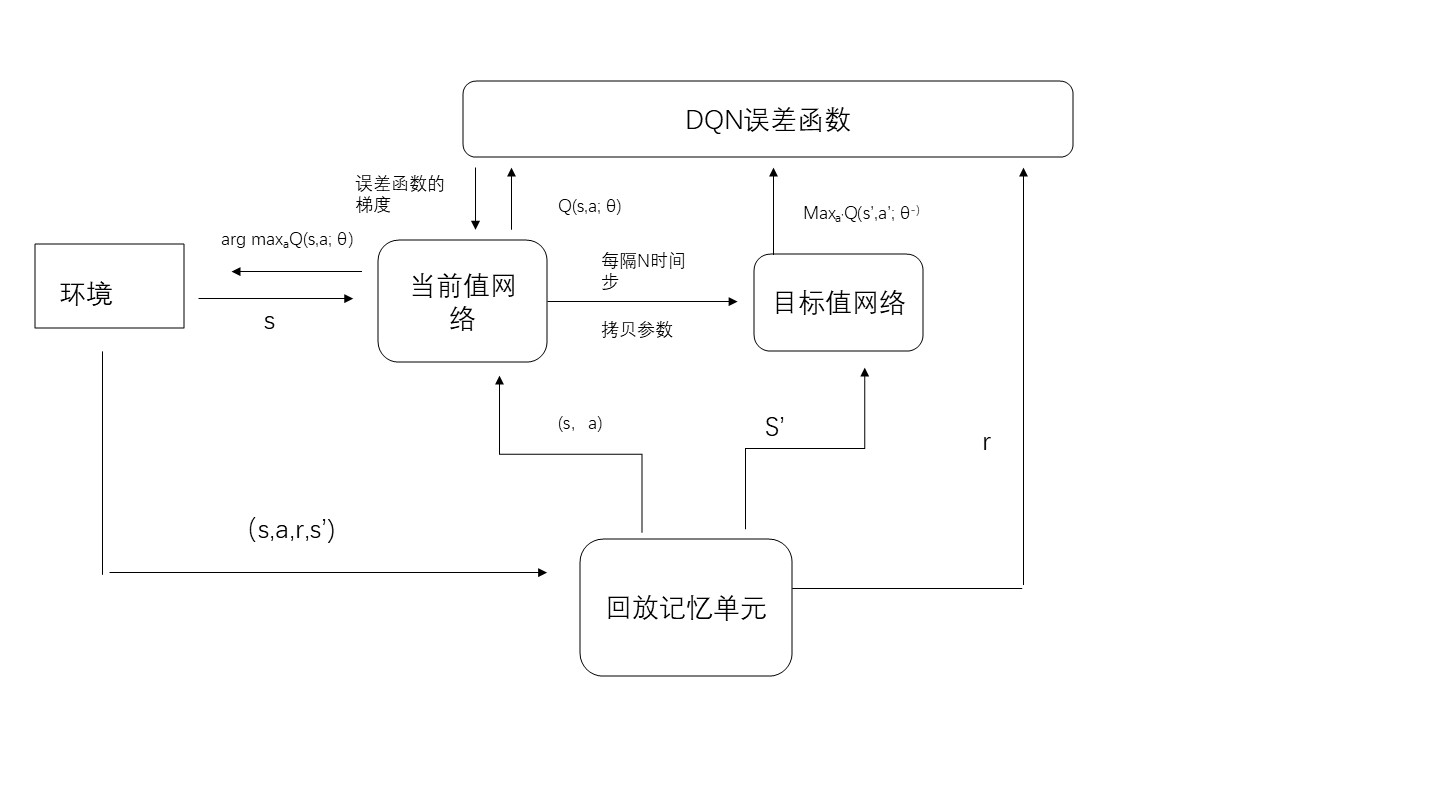
\includegraphics[width=\linewidth]{DQN算法模型训练过程.jpeg}
	\caption{DQN算法模型训练过程}
	\label{f.example}
\end{figure}

\subsection{深度Q网络算法经验池}

DQN 系统旨在使用内存设备来存储数据,通常称为内存缓存\cite{wawrzynski2013autonomous}。记忆装置能够储存相关信息,并解决前文提到的情境信息问题,从而满足认知障碍的标准。数据存储流程如下图3-3所示。

\begin{figure}[hbt]
	\centering
	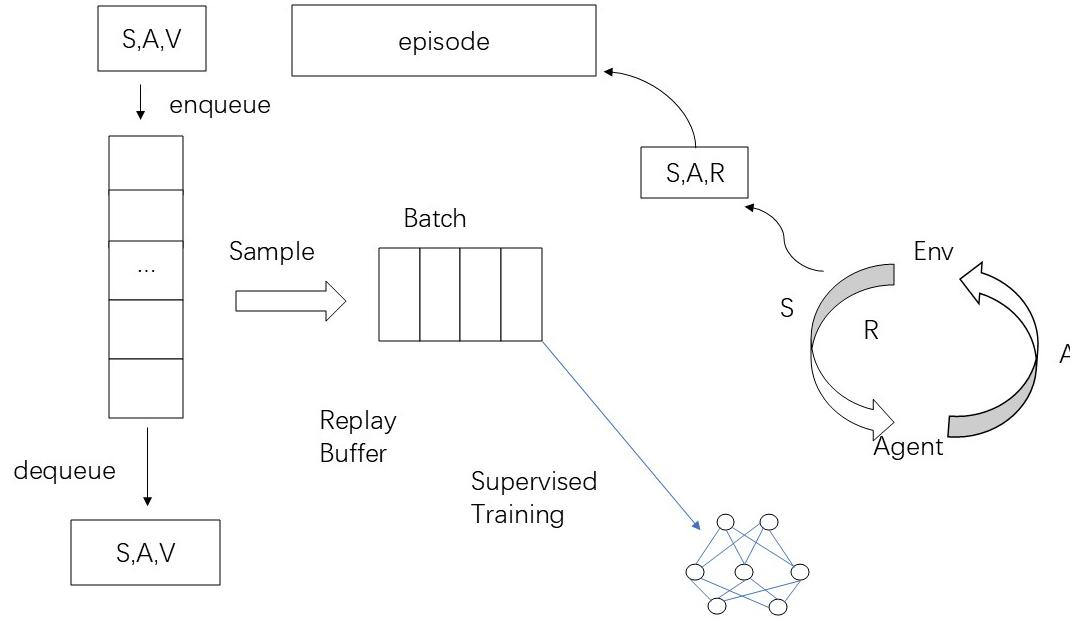
\includegraphics[width=\linewidth]{基于经验池机制的采样流程.jpeg}
	\caption{基于经验池机制的采样流程}
	\label{f.example}
\end{figure}

按照图3-3所示的工作流程,知识获取在Agent与环境的交互中起着重要作用。所有模板脚本都存储基本的关系信息。由于数据量巨大,观察者集群的存储容量必须足够大,才能持续收集和存储数据。在设计参与平台时,需要考虑许多因素,例如存储管理、配置和可用性。为了高效地存储结构化数据并将其存储在存储中,浏览器使用字符串或哈希表等结构化数据。集成系统使他们能够快速输入、移除和检索原材料以满足实时需求。

有两种看待它的方式。一个是曝光选择,另一个是曝光选择。在协作数据收集中,数据通常根据按时间顺序发生的事件进行收集。一旦大脑正确地记住了信息,它就会被覆盖,从而准确地再现之前呈现的信息。证据提取过程利用各种方法从大量事件中提取证据,然后进行检查和重建。此类操作可以提高您网站的性能。在上一节中,我们表明了智能游戏环境中交互得到的序列具有明确的时间关系,而任何通过空间学习得到的价值函数交互序列只能指向当前执行对应的下一条路径,而不能指向所有当前路径。
在这种情况下,如果网站没有跟上变化,它的外观就会与预期的外观产生差异。此外,随着协作学习的发展,方差将不断增加,这将对模型学习产生负面影响,例如增加模型的可变性并降低不变性。

DQN 工具作为一种综合工具,可针对大样本展开控制分析。相较于传统基于表格的教学方法而言,此方法在诸多方面呈现出改进态势。然而该方法存在较为严重的限制,即无法用于连续分析,并且当以神经学方式运用该药剂时,难以即刻达成习惯化,另外社交媒体的变革问题同样是需要尽快解决的。本节所阐述的 DQN 模型为后续发展的 DDPG 模型构建了基础,也为本文所提及的后续实验的成功开展提供了理论支撑。

\section{PPO 算法}

\subsection{PPO算法概述 }

从现有的研究可了解到,PPO属于强化学习的一种优化算法,它由OpenAI在2017年提出,主要针对策略梯度方法里学习不稳定、采样效率低的问题,PPO方案的主要思路是限制每个迭代周期内系统更新的次数,防止系统出现过多变化,让学习趋于稳定。PPO算法在信任体系中有易于实现、综合性更好等优势\cite{schulman2017proxima}。PPO算法能优化长期累积奖励,在需要进行长期规划和决策的高速公路驾驶场景中表现优异,这可使司机思考他们的长期目标,比如在高速公路上超速行驶以及右转或者保持在右车道行驶,PPO系统是基于网络的学习系统,可快速适应高速公路交通状况并给出实时反馈,PPO算法相较于PolicyGradient算法和TRPO算法有几个优点。其一数据选择过程和目标函数优化过程交替开展,标准策略梯度方法需更新每个数据样本的梯度,而PPO提供了新的目标函数,可对小组数据样本进行更新,其二和传统策略梯度相比,PPO能更高效地利用采样,其三与更复杂的TRPO相比,PPO更容易实现,且效果类似\cite{dey2017gate}。

从现有的研究中可发现,PPIO算法是基于策略搜索算法和宏观优化算法这两个主要算法构建的,依靠开展有意义的测试可看出,PPO可重复运用过去方法所生成的数据来对新方法给予指导,以此提升测试性能,剪枝技术借助减少更新策略的方式来提高学习准确率,防止因策略参数的突然变化而使性能得到提升。

\subsection{PPO算法原理 }

从现有的研究中可看出PPO算法属于在线策略算法,该算法主要处理的是连续动作空间里的高维度决策问题,它借助裁剪的概率比率来限定每次策略网络参数更新的幅度,以此让新策略比旧策略更具优势,PPO算法的更新步骤如下所示\cite{JSJJ20250416003}:

(1)采集样本数据,根据当前策略 $\pi$(a|s)执行若干次模拟,记录状态、动作、奖励和下一个状态。

(2)计算优势函数$𝐴_(t)$,计算公式如下:

\begin{align}
	Q_t(s_t, a_t) &= \sum_{s'} P(s' \mid s_t, a_t) \left[ R(s_t, a_t, s') + \gamma V_t(s') \right] \\
	V_t(s_t) &= \max_a Q_t(s_t, a) \\
	A_t &= Q_t(s_t, a_t) - V_t(s_t)
\end{align}

其中,\( Q_t(s_t, a_t) \) 是 \( Q \) 函数(动作价值函数),它表示在时间 \( t \) 采取动作 \( a_t \) 后从状态 \( s_t \) 开始的预期回报,其中 \( P(s' \mid s_t, a_t) \) 表示从状态 \( s_t \) 采取动作 \( a_t \) 转移到状态 \( s' \) 的概率,\( R(s_t, a_t, s') \) 是对应的奖励函数,\( \gamma \) 是折扣因子,\( V_t(s') \) 是状态 \( s' \) 的价值函数;\( V_t(s_t) \) 是价值函数,即在时刻 \( t \) 处于状态 \( s_t \) 的最大预期回报,通过最大化所有可能动作 \( a \) 的 \( Q \) 函数获得;优势函数 \( A_t \) 表示采取动作 \( a_t \) 相对于平均动作在状态 \( s_t \) 的额外回报。

(3)计算策略比率\(ratios\), 即新策略在状态 \( s_t \)下选择动作 \( a_t \)的概率与旧策略在状态 \( s_t \)下选择动作 \( a_t \)的概率的比值,计算公式如下:

\begin{equation}
	\text{ratio}_s = \frac{\pi_\theta(a_t \mid s_t)}{\pi_{\theta_k}(a_t \mid s_t)}
\end{equation}

(4)计算目标函数,使用剪裁函数\(𝑐𝑙𝑖𝑝(𝑟𝑎𝑡𝑖𝑜𝑠, 1 − 𝜖, 1 + 𝜖)\),将\(ratios\)的值限制在\([1 − 𝜖, 1 + 𝜖]\)的范围内,用于限制策略更新的幅度,根据公式上述计算如下:

\begin{equation}
	L(s, a, \theta_k, \theta) = \min\left( \text{ratios} \times A_t, \ \text{clip}\left( \text{ratios}, 1 - \epsilon, 1 + \epsilon \right) A_t \right)
\end{equation}

\(𝜃\)是当前策略参数,\(𝜃_𝑘\)是旧策略的参数;\(𝜖\)是超参数,指新策略和旧策略之间的更新幅度。

(5)通过优化目标函数来获得下一步策略参数\(𝜃_𝑘+1\),使用梯度下降法,公式见下:

\begin{equation}
	\theta_{k+1} = \arg\max_{\theta} \, \mathbb{E}_{s_a \sim \pi_{\theta_k}} \left[ L(s, a, \theta_k, \theta) \right]
\end{equation}

上面步骤中,步骤一的初始策略\(𝜋(𝑎|𝑠)\)就显得非常重要,强化学习算法的初始策略一般都是随
机策略,因为它可以提供更广泛的探索范围。

PPO 算法的具体结构图\cite{YYKX202405015}如图3-4所示。

\begin{figure}[hbt]
	\centering
	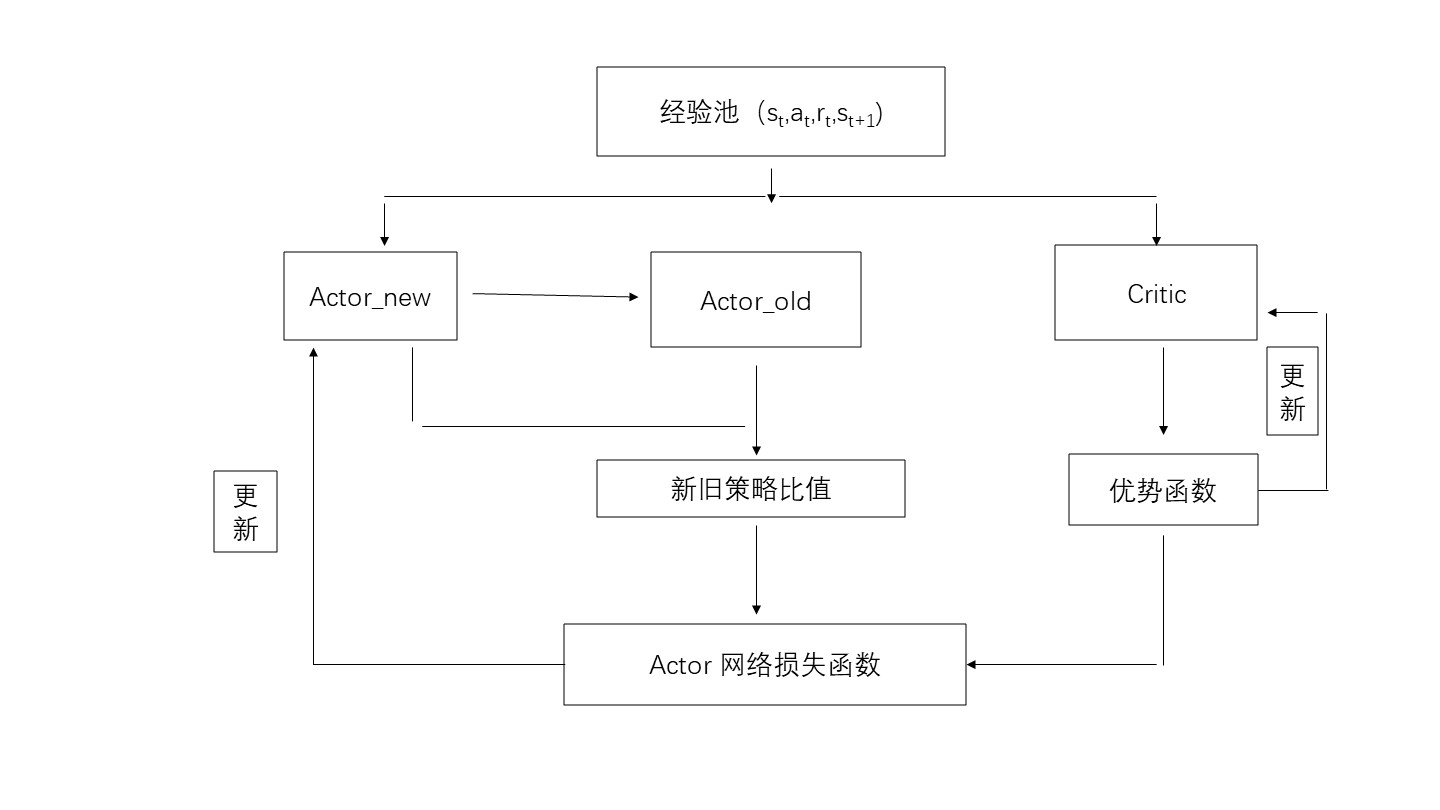
\includegraphics[width=\linewidth]{PPO算法结构图.jpeg}
	\caption{PPO算法结构图}
	\label{f.example}
\end{figure}

图 3-4 中的红色箭头表示前向传播模式的变化,蓝色箭头表示后向传播模式的改进。如图 3-4 所示,PPO 层次结构由两个参与者列表(\(actor_new\)和 \(actor_old)\)和动态流程组成。首先,在每个阶段,行动者网络根据当前状态 \(s_t\) 生成一个效用分布,然后代理根据这个效用分布做出贡献。然后状态根据代理每次动作为代理提供奖励值\(r_t\),移动到下一个状态\(s_t+1\),并生成数据序列\([s_t,a_t,r_t,s_t+1]\),存储在经验池中。一旦数据存储在特征池中,基于估计方法的类大小就会被传输并输入到 \(Actor_new\) 和 \(Critic\) 系统中进行训练。通过定期重复此过程,员工可以学习正确的技术。 \(Actor_new\)模块通过减少分解函数(包括新旧路径的速率以及检测函数)来更新其参数,而\(Critic\)模块通过发现函数来调整其参数,\(Actor_old\)模块通过不断复制\(Actor_new\)模块的参数来调整其参数。

\subsection{策略熵}

熵是衡量物体变化速率的指标。随着通道熵的增加,旧通道和自由基分布出现分歧。为了计算汽车值,我们通过计算熵值\cite{tucker2018mirage}来计算值的熵值,并计算值的熵系数(通常为0.01)。

\begin{align}
	H\big(\pi(\cdot \mid S_t)\big) &= -\sum_{a_i} \pi(a_i \mid S_t) \log \pi(a_i \mid S_t) \\
	&= \mathbb{E}_{a_i \sim \pi} \Big[ -\log \pi(a_i \mid S_t) \Big] \\
	&\sim e^{i\pi - k h_1 + \dots}
\end{align}

在强化学习中,策略熵的引入是一种有效的探索增强机制。连续作用的空间由积分描述。熵值越大,政策行动的分布越公平。因此,代理对不同行动的选择是任意的,而不是决定性的。在Actor-Critic架构中,加入政治熵作为Actor损失函数的先导,可以显著提高探索的效率。具体实现形式为:

\begin{align}
	H\big(\pi(\cdot \mid S_t)\big) &= -\sum_{a_i} \pi(a_i \mid S_t) \log \pi(a_i \mid S_t) \\
	&= \mathbb{E}_{a_i \sim \pi} \Big[ -\log \pi(a_i \mid S_t) \Big] \\
	&\sim e^{i\pi - k h_1 + \dots}
\end{align}

其中 \(L_policy\) 为原始策略梯度损失(如 PPO 的剪切目标函数),\(λ\)为熵系数(即 \(entropy_coef\),通常设为 0.01)。这种设计通过以下机制发挥作用:

(1)平衡探索与利用:

我们通过研究发现,熵正则化阶段不仅寻求策略优化中的更高回报(通过\(L_policy\)),而且还鼓励代理尝试更少的剥削行动。例如,在USV路径规划任务中,如果过程倾向于快速改进进化过程,则负的时间熵梯度将导致局部最优过程的概率分布发生倾斜,从而避免局部最优。

(2)自适应探索强度:

我们通过研究发现当训练开始时,系统熵增加,\(agent\)主动搜索环境;随着训练的进行,系统逐渐变得更加互联,熵自然减少,并且代理朝着使用更高奖励行动的方向发展。与固定次数的试验(如\(ε-greed\))相比,熵正则化具有更灵活的适应性,可以适应复杂的任务要求。

(3)实现简化与兼容性:
我们通过研究可以发现熵的计算直接基于现有策略的运行概率分布,不需要额外的环境干预或复杂的采样,并且易于与现有算法(例如PPO和SAC)集成。例如,在 PPO 的 Actor 更新中,仅需修改损失函数为:

\begin{equation}
	L^{\text{CLIP+Entropy}}(\theta) = \mathbb{E}_t \left[ \min\left( r_t(\theta) A_t, \ \text{clip}\left( r_t(\theta), 1-\varepsilon, 1+\varepsilon \right) A_t \right) \right] + \lambda \mathcal{H}(\pi_\theta)
\end{equation}

\subsection{优势归一化}

提高战略规划与当前环境条件的相关性;在进行车辆供应规划时,应利用广义需求估计(GAE)计算统计样本的需求函数,然后对整个细分市场的需求曲线进行标准化。归一化程序如下:首先,将网络中所有节点的初始聚合值居中对齐(平均值),并带有一个标准差(标准差);然后对每个需求价格进行标准变换,即减去平均单价,再除以单位标准差。这种扩展使得政治阶层体系更加稳定,消除了不同政党之间的阶层偏好差异,并增加了模型对当前行政分配形状的敏感性。初始最优值能清晰地显示出项目成本的优势与劣势;因此,要优化生产系统参数,需要根据实际环境条件,最终根据海况的变化,对项目进度进行优化。

\begin{equation}
	A^* = \frac{A - \mu}{\sigma}
\end{equation}

\section{SAC算法}

\subsection{SAC算法概述}
简单 Actor-Site 算法(SAC)\cite{zhou2022computation}是一种基于最大熵原理的强大的深度学习算法,是 Actor-Critic(AC)框架的重要发展。该算法在优化模型中引入单一策略熵作为正则表达式,在考虑多个预期奖励时最小化策略熵,从而在探索与探索之间建立强有力的平衡。设计帮助智能代理积极探索环境中的机会,同时避免因过度依赖历史经验而陷入局部最佳实践,并仍然追求长期利益。

基于其所构建的算法,SAC保留了“actor-critic”框架的基本思想,但引入了几项重要的创新。其关键电路采用两个Q决定因素(Q1和Q2),通过最小化两个独立比较器电路的误差来减少过冲问题,类似于双延迟DDPG设计(TD3)。具体来说,SAC实现了一种熵策略控制机制,通过温度参数\(α\)随机改变策略模式。在传统的强化学习算法中,当\( α\) 趋近于零时,它会减小,而随着 \(α\) 值的增加,策略变化会增加。这种设计有助于算法根据环境特征调整搜索强度。


经研究发现,SAC算法借助各类技术创新达成高质量且一致的学习,其一为契合学习连续函数需求,SAC算法运用迭代方式,将随机变量\(π(s|θ)\)除以不同噪声检测函数的乘积,策略通道输出动作方向\(μ\)与正态对数偏差\(σ\),依据公式\(μ+σ·ε(ε~N(0,1))\)生成最终动作。此设计遵循实用策略,又注重平滑的渐变过渡,其二SAC算法采用经验检索办法,把智能体与环境交互产生的过程存储于经验池中,借助随机排序阻断数据间的时序关系,提升了数据利用效率与持续学习能力。

\subsection{基于SAC的系统效益最大化算法}

从策略优化的视角出发可对SAC算法展开分析,SAC算法接受训练的目的在于优化最优策略效用函数\(J(π) = E[r(s,a)] + αH(π|s)\),这里面的\(H(π)\)所代表的含义是策略熵,借助逐步扩充参与者网络的方式提升实际性能,依靠最小化Q分数与目标值之间存在的微小误差对关键路径给予更新。需要留意的是,SAC算法运用一种简便的更新机制逐步调节输入至网络的参数,借此规避因突变致使的学习不稳定性,另外SAC算法运用“延迟策略回归”策略,于关键路径完全训练完毕之后对参与者网络进行更新,提升学习过程的稳定性。

可把SAC算法跟传统学习算法相互对比,连续SAC算法控制呈现出较为突出的性能优势,最大熵方法天然契合有多模态奖励或者强激励的环境,而重新参数化方法与基于经验的回归方法相结合,有效地化解了寻找继续行动之处的难题,从现有的研究可发觉,SAC算法在MuJoCo模拟环境里表现不错,在涉及细化的任务当中,其模型以及最终性能比其他强调相同时间的学习算法更具优势。SAC算法的这一特性在需要严格剖析的实际应用里颇为关键,比如机器人控制以及自动车辆控制,SAC算法中策略的优化目标可表示为:

\begin{align}
	\pi^* =& \operatorname*{argmax}_{\pi} \mathbb{E}_{(s_t, a_t) \sim p_{\pi}} \Bigg[ \sum_{t=0}^T \gamma^t \bigg( r(s_t, a_t, s_{t+1}) \\
	&+ \alpha H\big(\pi({\cdot} \mid s_t)\big) \bigg) \Bigg]
\end{align}

在上述公式里能发现,其中\(γ∈(0,1)\)是折扣率,此值直接体现代理人对长期回报的预期,当\(γ\) 靠近1时,该算法会优先顾及未来的奖励而非当前的奖励,这需要进行长期规划,像工业机器人的持续运行或者多阶段的投资决策,反之要是\(γ\)较小,代理很可能马上收到响应。这种方法在需要现实世界有变化或者环境条件发生重大改变的场景中颇为有用,\(γ\)的取值本质上呈现的是人类在不确定性条件下“选择时间”的行为,而数字的选择一般要考虑某些领域的先验知识来优化,上述公式中的\(α∈\)作为温度的函数,在工资函数和政策强度之间构建了一个新的权衡模型。从控制理论方面看,这个参数本质上是探索与开发权衡的驱动因素:随着 \(α\) 值增大,策略的熵权重增加,理性结构会找寻更昂贵但成本更低且潜在风险更高的决策分支,多学科护理变得越发关键,比如自动驾驶系统要应对所有意外的交通状况,然而当  \(α\) 趋于0时,算法会切换到传统的强化学习方法。在这些情形下,即便技术安全性有所提高,环境中的隐藏模式也可能无法被揭示,有意思的是,由于 \(α\) 基于学习,SAC算法能依据环境的复杂性自动调整搜索强度,这比\(ε-greedy\) 等默认搜索方法有一定优势。

和算法的基本公式相同,策略熵\(H(π(·|s))\)的物理概念相较于简单的知识概念度量而言,要复杂许多,从系统理论方面来看,熵最大化实际上是在功能空间里构建一个一致封闭的“可接受搜索空间”结构,此机制可让代理在状态空间的每个决策节点产生平均不确定性。当面对存在多种可能解决方案的问题时,高熵策略可避免过快收敛至局部最优解,而是可依靠创造性探索对剩余条件有局部的认识,该策略包含添加一个缓冲层来防止干扰,当面对环境变化时,分布式策略函数可提供多种解决方案,提高系统的整体性能,SAC借助把熵作为独立模块添加到局部目标活动中,达成了检测过程与策略优化的无缝整合,这比外部噪声活动检测方法有更大的理论吸引力和实际实现性。其中\(γ∈(0,1)\)是折扣率,其值直接体现代理人对长期回报的预期,当\(γ\)接近1时,该算法会优先考虑未来的奖励而非当前的奖励,这需要进行长期规划,比如工业机器人的持续运行或者多阶段的投资决策,相反若\(γ\)较小,代理很可能马上收到响应,这种方法在需要现实世界变化或环境条件发生重大变化的场景中非常有用。\(γ\)的取值本质上体现的是人类在不确定性条件下“选择时间”的行为,而数字的选择一般需要考虑某些领域的先验知识来优化。

SAC算法中的状态价值函数 \(V^π(s)\) 根据下式得到:

\begin{align}
	\overline{V^{\pi}(s)} 
	&= \mathbb{E}_{(s_t, a_t) \sim p_{\pi}} \Bigg[ \sum_{t=0}^{T} \gamma^t \bigg( r(s_t, a_t, s_{t+1}) \\
	&\quad + \alpha H\big(\pi({\cdot} \mid s_t)\big) \bigg) \,\bigg|\, s_0 = s \Bigg]
\end{align}
同时,动作状态价值函数\(Q_π( s,a)\)根据下式得到:

\begin{equation}
	\begin{aligned}
		Q^{\pi}(s, a) = \mathbb{E}_{(s_t, a_t) \sim p_{\pi}} \Bigg[ 
		\sum_{t=0}^{T} \gamma^t \bigg( &r(s_t, a_t, s_{t+1}) \\
		&+ \alpha \sum_{k=1}^{T} \gamma^k H\big(\pi({\cdot} \mid s_k)\big) \bigg) \Bigg| s_0 = s, a_0 = a \Bigg]
	\end{aligned}
\end{equation}

据以上分析,\(V^π( s)\) 和\(Q^π( s,a)\) 的关系可由下式表示:

\begin{equation}
	\begin{aligned}
		V^{\pi}(s) = \mathbb{E}_{z_{\hat{t}} \sim p} \Bigg[ 
		\mathbb{E}_{a_{\hat{t}} \sim \pi} \left[ Q^{\pi}(s_{\hat{t}}, a_{\hat{t}}) \right] 
		+ \alpha H\big(\pi({\cdot} \mid s_{\hat{t}})\big) 
		\Bigg]
	\end{aligned}
\end{equation}

\(Q^π( s,a)\)的贝尔曼期望方程也可以由下式表示:

\begin{align}
	Q^{\pi}(s, a) 
	&= \mathbb{E}_{s_{i+1} \sim p, a_{i+1} \sim \pi} \Big[ r(s_t, a_t, s_{i+1}) + \gamma \Big( Q^{\pi}(s_{i+1}, a_{i+1}) \nonumber \\
	&\quad + \alpha H\big(\pi({\cdot} \mid s_{i+1})\big) \Big) \Big] \nonumber \\
	&= \mathbb{E}_{s_{i+1} \sim p} \Big[ r(s_t, a_t, s_{i+1}) + \gamma V^{\pi}(s_{i+1}) \Big]
\end{align}

本研究基于针对上述问题开发的马尔可夫决策过程 (MDP) 模型,提出了基于软演员评论家 (SAC) 的视频流服务优化方法 SAC-UNCO。该算法通过高度强化的学习过程,可以更好地决策终端设备和外围服务器之间的动态视频任务传输。网络结构如图2所示。具体来说,SAC-UNCO采用五层网络架构,包括一个策略网络(actor network)、两个独立的Q值估计网络(critic 1和critic 2)以及两个匹配网络(target critic 1和target critic 2)。双组分 Q 值方案通过降低两个测试组合的最大值来消除 Q值估计过高的问题,同时,对所提出的组合进行简单的优化(Polak 平均)通过减少对组合参数的跟踪频率有效地提高了学习方法的稳定性。

为了在解决复杂问题的同时平衡传统动态研究中的研究和应用,SAC-UNCO 引入了自动训练的 \(α\) 温度。该参数根据策略网络参数通过梯度下降来动态调整策略熵权重,从而客观地控制策略网络的鲁棒性。具体而言,温度系数α的优化目标函数可表示为:

\begin{equation}
	L_{\alpha} = -\mathbb{E}_{\pi_{\phi}} \left[ \alpha \log \pi_{\phi}(a \mid s) \right] + \beta \cdot \text{regularizer}
\end{equation}

我们可以通过上述公式发现,前者被鼓励利用政治熵进行研究,而后者的典型约束则防止\(α\)增长过快导致政策分歧。自动温度控制使得算法能够完全根据环境因素调整搜索力度,而无需输入搜索参数,大大提高了算法适应复杂视频提取场景的能力。

我们可以发现在训练的过程中,SAC-UNCO使用档案重放来存储历史交互数据并锁定跨模型数据之间的时间相关性,从而提高该模型的可用性。规则网络利用重参数化的方法对不同任务中执行的随机动作进行变换,从而利用反向传播的方法优化规则系数。同时,双拟合优度网络利用损失误差函数方程,通过减少与目标值Q的差异来调整网络参数。其中目标Q值由贝尔曼方程定义并融入策略熵项:

\begin{equation}
	y = r + \gamma \cdot \min_{i=1,2} Q_{\theta_i}\big(s', \pi_\phi(s')\big) - \alpha \log \pi_\phi(a \mid s')
\end{equation}

我们可以通过上述公式发现,在该过程允许进行成本效益分析,以评估即时回报和长期利益,以及比较重复的矿物开采机会。实验表明,SAC-UNCO 优于传统的视频性能测试方法。它的动态分析可以管理网络流量和计算资源的路由,同时降低速度和能耗并提高性能。算法中的 Q 值网络、策略网络和温度系数自动调节的细节如图3-5所示。

\begin{figure}[hbt]
	\centering
	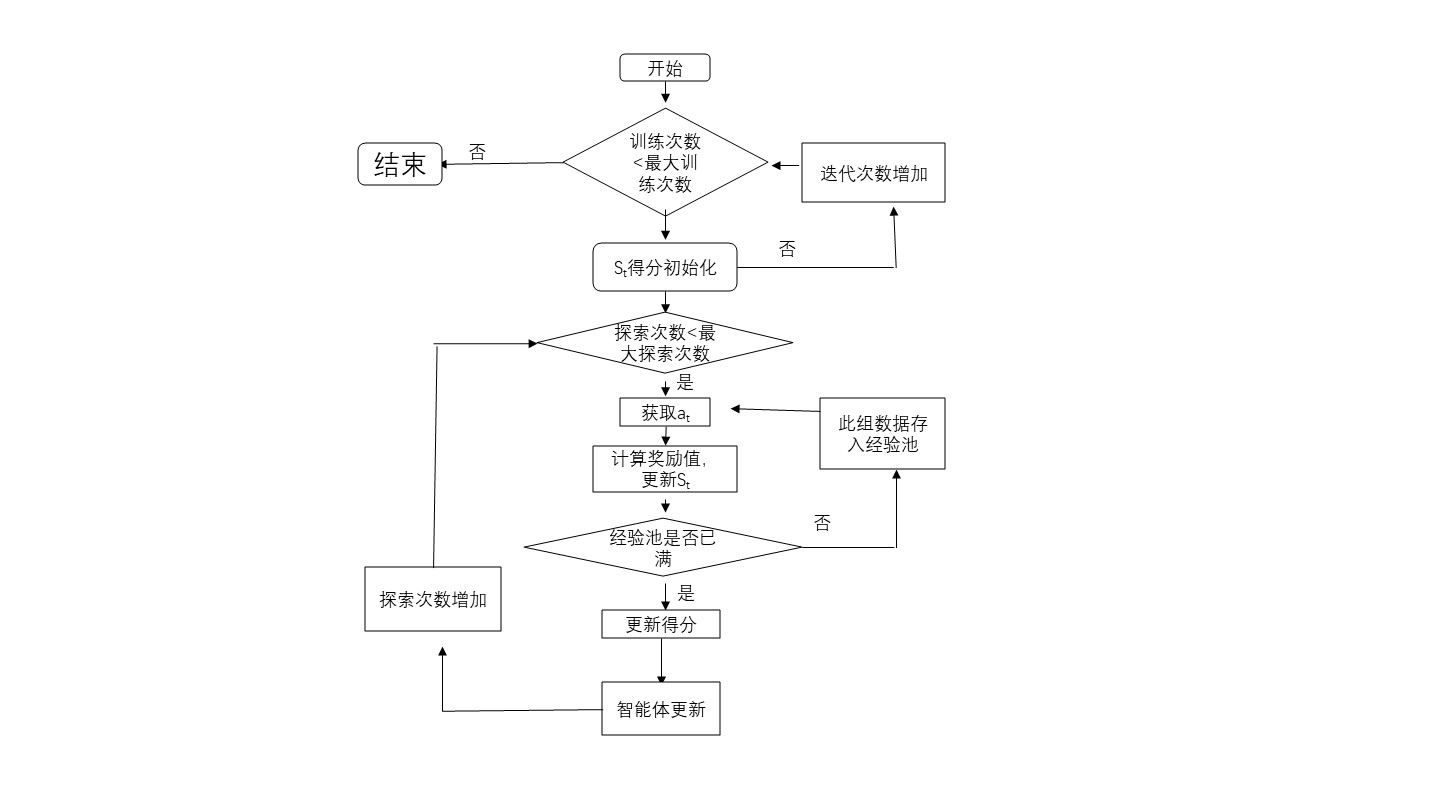
\includegraphics[width=\linewidth]{SAC算法训练架构.jpeg}
	\caption{SAC算法训练架构}
	\label{f.example}
\end{figure}


\subsection{Q值网络}

在本篇文章的研究中,为了正确估计强化学习中的状态和动作价值函数\(Q(s,a)\),本研究采用了参数为\(β_i\)的神经网络。就具体的来说,对于每个状态-动作对 (s, a),其 Q 值可以表示为神经网络的输出 \(Q_(β_i)(s, a)\),其中 \(i∈[1,2]\) 表示神经网络的两个独立参数。该设计包括用于实时策略评估和目标计算的两层网络结构,从而解决了传统单网络方法中常见的高估问题。

此外,我们在优化参数时,该算法使用均方误差(MSE)损失函数作为主要指标。对于不考虑网络的情况,损失函数 \(L(β_i)\) 由下式定义:

\begin{equation}
	\begin{split}
		J_{Q}(\beta_{i}) 
		&= \mathbb{E}_{(s_i, a_i, s_{i+1}) \sim D} \bigg[ \frac{1}{2} \Big( Q_{\beta_i}(s_i, a_i) \\
		&\quad - \hat{Q}(s_i, a_i) \Big)^2 \bigg]
	\end{split}
\end{equation}

在SAC-UNCO算法中,状态-动作价值函数Q\(^π(st,at)\)的更新过程遵循改进的贝尔曼方程,其表达式为:

\begin{equation}
	Q^{\pi}(s_t, a_t) = r(s_t, a_t) + \gamma \left( Q_{\beta_i}(s_{t+1}, a_{t+1}) - \alpha \log \pi_{\theta}(a_{t+1} \mid s_{t+1}) \right)
\end{equation}

这里\(r(s_t,a_t)\)表示代理在时间 t 执行动作后的即时奖励,\(γ∈(0,1)\)是用于衡量未来奖励对当前决策影响的折扣因子。具体来说,该公式使用了基于传统贝尔曼方程的 \(−αlog⁡πθ(a_t+1|s_t+1)\) 阶熵项,其中 \(α\) 是可测量的温度系数,\(π_θ\)是限制于 \(θ\)的晶格阶。熵概念的引入包含了研究熵的最大能量的基本思想。通过明确鼓励策略中的随机性,鼓励代理探索环境中的机会,同时增加其积累的奖励。这提高了算法适应动态情况的能力。

借助研究可明白,经验丰富的D重复池可作为算法学习点,其持续收集代理与环境交互产生的轨迹数据\((s_t,a_t,r_t,s_t+1)\),借助均匀随机采样打破数据间的时间联系,这种在线学习方法有效降低了模型相关性,避免了多个相似模型引发的梯度漂移问题,还借助重新处理数据大幅提升了建模效率。池中存储的值\(Q_(β_i)(s_t+1,a_t+1)\)并非由当前网络直接计算,而是由目标Q值网络近似确定,扩展参数\(β_i\)按软更新规则)更新,采用指数移动平均策略逐步更新目标网络参数:\(β_i′​←τβ_i′​+(1−τ)β_i(τ≪1τ≪1)\)。这种延迟更新机制有效解决了Q值估计与目标值波动耦合的问题,为策略优化提供了稳定参考点。
\begin{align}
	\overline{\beta_i} &= \tau \beta_i + (1 - \tau) \overline{\beta_i}
\end{align}

根据式(3.29)可以得到Q值的梯度\(∇_(β_i) (j_Q)( β_i)\)表示为:

\begin{equation}
	\nabla_{\beta_i'} J_Q(\beta_i) = \nabla_{\beta_i'} Q_{\beta_i}(s_t, a_t) \left( \widetilde{Q_{\beta_i}(s_t, a_t)} - \hat{Q}(s, a) \right)
\end{equation}

因此,Q 值网络在时隙t的网络参数 \(β_i\) 可以根据式(3.32)更新

\begin{align}
	\beta_{i}^{t+1} &= \beta_{i}^{t} - \lambda_{\beta} \nabla_{\beta_{i}} J_{Q}(\beta_{i})
\end{align}

其中:\(λ_β\) 是Q值网络的学习率。































